\documentclass[12pt]{jarticle}
\usepackage{comment}
\usepackage{braket}
\usepackage{fullpage}
\usepackage{float}
\usepackage{color}
\usepackage{multicol}
\usepackage[dvipdfmx]{pict2e}
\usepackage{wrapfig}
\usepackage{graphicx}
\usepackage{bm}
\usepackage{url}
\usepackage{underscore}
\usepackage{colortbl}
\usepackage{tabularx}
\usepackage{fancyhdr}
\usepackage{ulem}
\usepackage{cite}
\usepackage{amsmath,amssymb,amsfonts}
\usepackage{hyperref}
\usepackage{algorithmic}
\usepackage{textcomp}
\usepackage{xcolor}
\usepackage[ipaex]{pxchfon}


\begin{document}

\title{Hubbard模型}
\author{Koki Shimura}
\maketitle

バンド理論において、多数の電子の間にはたらくクーロン斥力(電子相関)はいったん平均化され、周期ポテンシャル$V(r)$のみが考慮して取り扱われている。これを一体近似という。バンド理論の成功により、電子相関を考慮しなくても金属・絶縁体の区別がおおかた可能であることが明らかになった。つまり大抵の場合は一体近似で事足りるのである。では電子相関が重要になるのはどのような場合であろうか。

バンド理論によれば、ユニットセルあたりの電子が奇数個である場合、バンドをスピン$\uparrow$と$\downarrow$の電子で部分的にしか詰めることができず、反対のスピンを持つ電子を詰める余地が必ず存在するために、系は必ず金属的になる。実はこの結論に矛盾する絶縁体が存在する。特に遷移金属酸化物の例が有名である。例えばコバルト酸化物CoOは、酸素原子が8個、コバルト原子が27個の電子をもつため、ユニットセルあたりの電子の個数は奇数になる。それにもかかわらず、CoOは絶縁性を示す。同様の事情は、Mnが25個の電子を持つMnOにも当てはまる。本事象には電子相関が重要な役割を果たしていると考えられており、それを記述するミニマムな模型としてHubbard模型が存在する。

\section{Hubbard模型のハミルトニアン}
Hubbard模型のハミルトニアン$\mathcal{H}$は以下で与えられる。
\begin{equation}
  \mathcal{H} = \sum_{i,j} (t_{ij} c_{i}^\dagger c_{j} + h.c.) + U\sum_{i}n_{i\uparrow}n_{i\downarrow}
  \label{Hubbard}
\end{equation}
$t_{i,j}$はサイトi,jの間の飛び移り積分である。$c_{i}$($c_{i}^{\dagger}$)はサイトiの電子の消滅(生成)演算子であり、$n_{i\uparrow}$($n_{i\downarrow}$)はサイトiにおけるスピン$\uparrow$($\downarrow$)の電子の個数演算子である。第2項を見ると分かるように、$n_{i\uparrow}$, $n_{i\downarrow}$の取りうる値は0か1であり、電子間のクーロン斥力は電子が同一サイトにあるときのみ働く。

Hubbard模型におけるパラメータは以下のとおりである。
\begin{itemize}
  \item 電子のホッピング$t_{i,j}$
  \item クーロン斥力U
  \item 電子の個数
  \item 系の次元・結晶構造
\end{itemize}

Hubbard模型は大胆な近似に基づいている。例えば、クーロン斥力は本来長距離相互作用であるが、本模型では異なるサイト間でクーロン力は一切働かないとしている。また固体中でしばしば重要になる軌道自由度も考慮されていない。それにも関わらず、Hubbard模型は固体電子のふるまいをかなりよく記述する。それは単にバンド理論で説明できない金属・絶縁体の区別を明確にするだけでなく、磁性や高温超伝導の議論まで行うことができる。これほどまでに単純化された模型から多彩な物理が表れることは驚くべきことである。Hubbard模型の物理を余すことなく記述するのは、筆者の手に余る大事業であるので、ここでは金属・絶縁体を区別する観点から論じていく。

\section{Heisenbergハミルトニアンの導出}
Hubbard模型は単純な模型ながら、2次元以上の場合には完全に解明されているとは言い難い。一方でハーフフィリングの物理は多くのことが分かっており、解析計算でたどり着ける結論もある。ここではクーロン斥力$U$が強く、ホッピング$t$が摂動として扱える場合、すなわち$U/t \gg 1$とみなせる場合を考える。まどろっこしい説明にはなるが、無摂動ハミルトニアン$\mathcal{H}^{'}$は、各サイトに電子が0から2個存在しているものの、サイト間の行き来はないような状態に対応している。ここに$\mathcal{H}$を加えて、電子間の移動を摂動として考慮した場合の有効ハミルトニアンが知りたい。量子力学によれば、2次摂動の演算子は
\begin{equation}
  \mathcal{H}^{(2)} = \mathcal{H}_0 \frac{1}{E_0 - \mathcal{H}^{'}}\mathcal{H}_0
  \label{second perturbation}
\end{equation}
で与えられるので、式(\ref{Hubbard})を代入すると

\begin{eqnarray*}
\mathcal{H}^{(2)}
=
-\frac{t^2}{U}
\sum_{\langle i,j\rangle}\sum_{\sigma,\sigma'}
\Bigl(
   c_{1\uparrow}^\dagger c_{2\uparrow}
 + c_{2\uparrow}^\dagger c_{1\uparrow}
 + c_{1\downarrow}^\dagger c_{2\downarrow}\,
 + c_{2\downarrow}^\dagger c_{1\downarrow}
\Bigr)^2
\end{eqnarray*}
となる。今サイト1にスピン$\uparrow$の電子が、サイト2にスピン$\downarrow$の電子がいると仮定する。この状態は電子がいない状態を$\ket{0}$として$c_{1\uparrow}^\dagger c_{2\downarrow}^\dagger\!\ket{0}$と表せる。2次摂動のハミルトニアンを作用させると

\begin{eqnarray}
  \mathcal{H}^{(2)}
c_{1\uparrow}^\dagger c_{2\downarrow}^\dagger\!\ket{0}
\;&=&\;
-\frac{t^2}{U}\,
\Bigl(
   c_{1\uparrow}^\dagger c_{2\uparrow}
 + c_{2\uparrow}^\dagger c_{1\uparrow}
 + c_{1\downarrow}^\dagger c_{2\downarrow}\,
 + c_{2\downarrow}^\dagger c_{1\downarrow}
\Bigr)^2\,
c_{1\uparrow}^\dagger c_{2\downarrow}^\dagger\!\ket{0} \notag\\
\;&=&\;
-\frac{t^2}{U}\,
\Bigl(
   c_{1\uparrow}^\dagger c_{2\uparrow}
 + c_{2\uparrow}^\dagger c_{1\uparrow}
 + c_{1\downarrow}^\dagger c_{2\downarrow}\,
 + c_{2\downarrow}^\dagger c_{1\downarrow}
\Bigr)\,
\Bigl(c_{1\uparrow}^\dagger c_{1\downarrow}^\dagger+c_{2\uparrow}^\dagger c_{2\downarrow}^\dagger\Bigr)\!\ket{0} \notag\\
\;&=&\;
-\frac{2t^2}{U}\,
\Bigl(c_{1\uparrow}^\dagger c_{2\downarrow}^\dagger-c_{2\uparrow}^\dagger c_{1\downarrow}^\dagger\Bigr)\!\ket{0}\\
\end{eqnarray}
となる。最後の式は、2次摂動によってサイト1にいた電子とサイト2にいた電子が元に戻る場合、互いに入れ替わる場合の線形結合である。

ここでやや天下りではあるが、スピン演算子
\begin{equation}
S_i^z = \frac12\bigl(c_{i\uparrow}^\dagger c_{i\uparrow} - c_{i\downarrow}^\dagger c_{i\downarrow}\bigr), 
\quad
S_i^+ = c_{i\uparrow}^\dagger c_{i\downarrow}, 
\quad
S_i^- = c_{i\downarrow}^\dagger c_{i\uparrow}.
\label{spinop}
\end{equation}
を導入する。この時スピン演算子の内積は
\begin{equation}
  \vec S_1 \cdot \vec S_2
= S_1^z S_2^z + \frac12 \bigl(S_1^+ S_2^- + S_1^- S_2^+\bigr)
\end{equation}
で与えられるから、式(\ref{spinop})を代入すると

\begin{equation}
  \vec S_1 \cdot \vec S_2
= \frac14\,(n_{1\uparrow}-n_{1\downarrow})(n_{2\uparrow}-n_{2\downarrow})
+ \frac12\Bigl(
  c_{1\uparrow}^\dagger c_{1\downarrow}\,c_{2\downarrow}^\dagger c_{2\uparrow}
+ c_{1\downarrow}^\dagger c_{1\uparrow}\,c_{2\uparrow}^\dagger c_{2\downarrow}
\Bigr)
\end{equation}
これを最初の状態$c_{1\uparrow}^\dagger c_{2\downarrow}^\dagger\ket{0}$に作用させると
\begin{eqnarray}
  \vec S_1\cdot\vec S_2 \;c_{1\uparrow}^\dagger c_{2\downarrow}^\dagger\ket{0}
&=& \frac{1}{4}\Bigl(2c_{1\downarrow}^\dagger c_{1\uparrow}c_{2\uparrow}^\dagger c_{2\downarrow} - c_{1\uparrow}^\dagger c_{1\downarrow}c_{2\downarrow}^\dagger c_{2\uparrow}\Bigr)c_{1\uparrow}^\dagger c_{2\downarrow}^\dagger\ket{0} \notag\\
&=&\Bigl(-\frac{1}{4}c_{1\uparrow}^\dagger c_{2\downarrow}^\dagger+\frac{1}{2}c_{2\uparrow}^\dagger c_{1\downarrow}^\dagger\Bigr)\!\ket{0}
\end{eqnarray}
となる。式(12)式の辺々から$\frac{1}{4}c_{1\uparrow}^\dagger c_{2\downarrow}^\dagger\!\ket{0}$
を引くと
\begin{equation}
  \bigl(\vec S_1\cdot\vec S_2 - \frac{1}{4}\bigr) \;c_{1\uparrow}^\dagger c_{2\downarrow}^\dagger\ket{0} = -\frac{1}{2}\,
\Bigl(c_{1\uparrow}^\dagger c_{2\downarrow}^\dagger-c_{2\uparrow}^\dagger c_{1\downarrow}^\dagger\Bigr)\!\ket{0} = \frac{U}{4t^2}\mathcal{H}^{(2)}
c_{1\uparrow}^\dagger c_{2\downarrow}^\dagger\!\ket{0}
\end{equation}
となる。従って
\begin{equation}
  \mathcal{H}^{(2)} = 2J\bigl(\vec S_1\cdot\vec S_2 - \frac{1}{4}\bigr) \qquad J = \frac{2t^2}{U}>0
\end{equation}
となる。この2次摂動の意味は、スピンが反平行$\bigl(\vec S_1\cdot\vec S_2 = -\frac{1}{4}\bigr)$のときにエネルギーが低下するが、平行な場合は遷移がないことを意味している。これはパウリの排他律とも一致している。定数項を落として
\begin{equation}
  \mathcal{H}_{eff} = 2J\bigl(\vec S_1\cdot\vec S_2 \bigr)
\end{equation}
と書けば、この有効ハミルトニアン$\mathcal{H}_{eff}$が反強磁性Heisenbergモデルになっていることもわかる。モット絶縁体における有効ハミルトニアンは反強磁性Heisenberg模型である。

\section{Hubbard \rm{I}}
ハーフフィリング以外の場合にどのような物理が表れるかは未解明の部分も多く、様々な近似計算に基づいた数値計算が行われる。実際模型の提案された論文で既に状態密度の近似計算手法が紹介されていて、現在ハバード1と呼ばれている。まず原子極限のグリーン関数$G^a(\omega)$について述べ、次に$G^a(\omega)$を用いた自己エネルギーの構築と状態密度の計算手法について述べる。
\subsection{原子極限のグリーン関数}
飛び移り積分がクーロン斥力に比べて極めて小さく、$t_{i,j} = 0$とみなせるような場合を原子極限(atomic limit)と呼ぶ。サイトiにおける原子極限のハミルトニアンは
\begin{align}
  \mathcal{H}_{\rm atom}
  &= U\,n_{i\uparrow}n_{i\downarrow}
\end{align}
と書ける。

ここでレーマン表示のグリーン関数は
\begin{align}
  G_0(i\omega_n)
  &= \frac{1}{Z}
     \sum_{m,n}
     \frac{e^{-\beta E_n} + e^{-\beta E_m}}
          {i\omega_n + E_n - E_m}
     \bigl|\langle m|\,c_{i\sigma}^\dagger\,|n\rangle\bigr|^2 \notag
  \\
  &= (1-n)\,\frac{1}{i\omega_n - ( -\mu )}
     + n\,\frac{1}{i\omega_n - (U-\mu)} \notag
  \\
  &= \frac{1-\langle n_{-\sigma} \rangle}{\,i\omega_n+\mu\,}
     +\frac{\langle n_{-\sigma} \rangle}{\,i\omega_n+\mu - U\,}.
\end{align}
である。これを解析接続することによって、原子極限のグリーン関数が
\begin{equation}
  G_0(\omega) = \frac{1-\langle n_{-\sigma} \rangle}{\omega + i\delta}
     +\frac{\langle n_{-\sigma} \rangle}{\omega - U+i\delta\,}
\end{equation}
と与えられる。

\begin{figure}[h]\label{fig:atomic-limit}
  \centering
  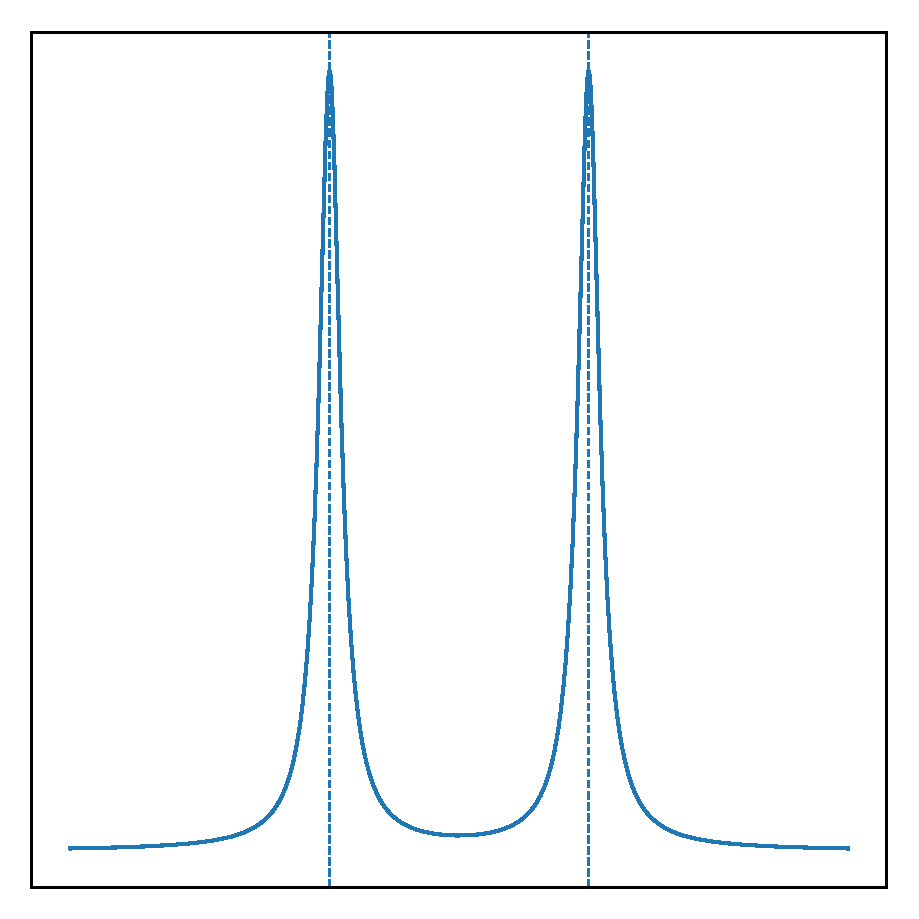
\includegraphics[width=0.3\textwidth]{dos_atomic_limit_square.eps}
  \caption{原子極限における状態密度。化学ポテンシャルが$E_d + \omega > \mu$かつ$E_d < \mu$にあるとき、系は絶縁体になる。}
\end{figure}

\subsection{自己エネルギーの導出}
Hubbardは原子極限のグリーン関数$G^a(\omega)$を用いて、グリーン関数を

\section{Hubbard \rm{I}\hspace{-1pt}\rm{I}\hspace{-1pt}\rm{I}}


\begin{thebibliography}{9}
  \bibitem{hofstadter} Hofstadter, Douglas R., Energy levels and wave functions of Bloch electrons in rational and irrational magnetic fields, Phys. Rev. B $\bm{14}$, 2239(1976).
  \bibitem{super} C R Dean 1, L Wang, P Maher, C Forsythe, F Ghahari, Y Gao, J Katoch, M Ishigami, P Moon, M Koshino, T Taniguchi, K Watanabe, K L Shepard, J Hone, P Kim, Hofstadter's butterfly and the fractal quantum Hall effect in moiré superlattices, Nature 497(7451), (2013)
\end{thebibliography}


\end{document}